%%% To fix widows and orphans, see:
%https://en.wikibooks.org/wiki/LaTeX/Page_Layout#Widows_and_orphans

%----------------------------------------------------------
%
\documentclass[letterpaper,12pt,openany,reqno]{book}%

%
%----------------------------------------------------------
% This is a sample document for the standard LaTeX Book Class
% Class options
%       --  Body text point size:
%                        10pt (default), 11pt, 12pt
%       --  Paper size:  letterpaper (8.5x11 inch, default)
%                        a4paper, a5paper, b5paper,
%                        legalpaper, executivepaperF
%       --  Orientation (portrait is the default):
%                        landscape
%       --  Printside:   oneside, twoside (default)
%       --  Quality:     final(default), draft
%       --  Title page:  titlepage, notitlepage
%       --  Columns:     onecolumn (default), twocolumn
%       --  Start chapter on left:
%                        openright(no, default), openany
%       --  Equation numbering (equation numbers on right is the default):
%                        leqno
%       --  Displayed equations (centered is the default):
%                        fleqn (flush left)
%       --  Open bibliography style (closed bibliography is the default):
%                        openbib
% For instance the command
%          \documentclass[a4paper,12pt,reqno]{book}
% ensures that the paper size is a4, fonts are typeset at the size 12p
% and the equation numbers are on the right side.
%
\usepackage{amsmath}%
\usepackage{amsfonts}%
\usepackage{amssymb}%
\usepackage{graphicx}
\usepackage{subcaption}
\usepackage[colorlinks=true,linkcolor=blue]{hyperref}
%\hypersetup{pdfauthor={Philip Howard}, pdftitle={A Very Simple Compiler Book}}

\usepackage{tikz}
\usetikzlibrary{shapes,arrows}

\usepackage{float}
\floatstyle{boxed} 
\restylefloat{figure}

\newfloat{mylisting}{thbp}{lob}[chapter]
\floatname{mylisting}{Listing}

\usepackage{listings}
\lstset{ %
xleftmargin={0.5in},						% left margin
language=C,                			% choose the language of the code
columns=flexible,
basicstyle=\small\ttfamily,     % the size of the fonts that are used for the code (was sffamily)
numbers=left,                   % where to put the line-numbers
numberstyle=\small,             % the size of the fonts that are used for the line-numbers
stepnumber=5,                   % the step between two line-numbers. If it's 1 each line will be numbered
numberfirstline=true,						% number the first line of the listing
firstnumber=1,									% auto or <number>
numbersep=5pt,                  % how far the line-numbers are from the code
%backgroundcolor=\color{white},  % choose the background color. You must add \usepackage{color}
showspaces=false,               % show spaces adding particular underscores
showstringspaces=false,         % underline spaces within strings
showtabs=false,                 % show tabs within strings adding particular underscores
frame=single,	                  % adds a frame around the code
tabsize=2,	                    % sets default tabsize to 2 spaces
captionpos=b,                   % sets the caption-position to bottom
breaklines=true,                % sets automatic line breaking
float=thbp,
%breakatwhitespace=false,        % sets if automatic breaks should only happen at whitespace
%title=\lstname,                 % show the filename of files included with \lstinputlisting; also try caption instead of title
%escapeinside={\%*}{*)}            % if you want to add a comment within your code
}


\lstnewenvironment{derivation}[2]
{
\lstset{float=thbp,caption={#1},label={#2},numbers=none}
\renewcommand{\lstlistingname}{Derivation}
}
{
\lstset{numbers=left}
\renewcommand{\lstlistingname}{Listing}
}

\lstnewenvironment{cfg}[2]
{
\lstset{float=thbp,caption={#1},label={#2},stepnumber=1,escapechar=Q}
\renewcommand{\lstlistingname}{CFG}
}
{
\lstset{numbers=left,stepnumber=5}
\renewcommand{\lstlistingname}{Listing}
}

\newcommand{\code}[1] {\lstinline[breaklines=yes,breakatwhitespace=yes]{#1}}

\newcommand{\cfgprod}[2] {\ttfamily{#1} $\rightarrow$ \ttfamily{#2}}

%\usepackage[T1]{fontenc}  % access \textquotedbl
%\usepackage{textcomp}     % access \textquotesingle

\newcommand{\needswork}{\paragraph{This section needs work.}}
\newcommand{\needsproblems}{\paragraph{Add practice problems here.}}

%---------------------------------------------------
% commands for drawing FAs
\usetikzlibrary{arrows.meta} % to specify arrow size in transition commands.
\newcommand{\faterminalnode}[3] {\draw (#1) circle [radius=9pt]; \node at (#1) (#2) [circle, draw, minimum size=24pt] {#2};}
\newcommand{\fastart}[1] {\coordinate (start) at (#1);}
\newcommand{\fanonterminalnode}[2] {\node at (#1) (#2) [circle, draw, minimum size=24pt] {#2};}
\newcommand{\fanolabel}[2] {\node at (#1) (#2) [circle, draw, minimum size=24pt] {};}
\newcommand{\fatransition}[3] {\draw [-{Latex[length=3mm,width=2.5mm]}] (#1) -- (#2) node [midway, above] {#3};}
\newcommand{\farighttransition}[3] {\draw [-{Latex[length=3mm,width=2.5mm]}] (#1) -- (#2) node [midway, right] {#3};}
\newcommand{\faarctransition}[5] {\draw [-{Latex[length=3mm,width=2.5mm]}] (#1) to[out=#4, in=#5] node  [midway, above] {#3} (#2) ;}
%---------------------------------------------------

\usepackage{mdwlist}
\newenvironment{mydesc}[1][9em]
  {
     \begin{basedescript}
     {
      \renewcommand{\makelabel}[1]{\bfseries##1}
      \desclabelwidth{ #1 }
      \desclabelstyle{\multilinelabel}
     }
  }
  {
     \end{basedescript}%
  }
\makecompactlist{mydesc*}{mydesc}

%----------------------------------------------------------
\newtheorem{theorem}{Theorem}
\newtheorem{acknowledgement}[theorem]{Acknowledgement}
\newtheorem{algorithm}[theorem]{Algorithm}
\newtheorem{axiom}[theorem]{Axiom}
\newtheorem{case}[theorem]{Case}
\newtheorem{claim}[theorem]{Claim}
\newtheorem{conclusion}[theorem]{Conclusion}
\newtheorem{condition}[theorem]{Condition}
\newtheorem{conjecture}[theorem]{Conjecture}
\newtheorem{corollary}[theorem]{Corollary}
\newtheorem{criterion}[theorem]{Criterion}
\newtheorem{definition}[theorem]{Definition}
\newtheorem{example}[theorem]{Example}
\newtheorem{exercise}[theorem]{Exercise}
\newtheorem{lemma}[theorem]{Lemma}
\newtheorem{notation}[theorem]{Notation}
\newtheorem{problem}[theorem]{Problem}
\newtheorem{proposition}[theorem]{Proposition}
\newtheorem{remark}[theorem]{Remark}
\newtheorem{solution}[theorem]{Solution}
\newtheorem{summary}[theorem]{Summary}
\newenvironment{proof}[1][Proof]{\textbf{#1.} }{\ \rule{0.5em}{0.5em}}
%----------------------------------------------------------
\begin{document}

\frontmatter
\title{A Very Simple Grammars Book}
\author{Philip W. Howard}
\date{\today}
\maketitle
\tableofcontents
\listoffigures
\chapter{Preface}
I've been teaching Introduction to Grammars (aka Computer Theory) at Oregon Institute of Technology (OIT) for several years. OIT offers a very hands-on program, so why include a theory course?

There is a Computer Theory text that I really like, but it has become criminally expensive (as I'm writing this, Amazon would be glad to sell you a new paperback edition for over \$300). So, why not write my own? Lot's of reasons that I won't enumerate, but obviously I've attempted to get past those and actually write the book. 

\needswork

I hope that this book proves useful to my students, and if it is discovered by others, that it is useful to them as well.

Phil Howard
\mainmatter
%%%%%%%%%%%%%%%%%%%%%%%%%%%%%%%%%%%%%%%%%%%%%%%%%%%%
%% FORMATTING
\setlength{\parindent}{0cm} % Default is 15pt.
\setlength{\parskip}{12pt plus 2pt minus 2pt}
%%%%%%%%%%%%%%%%%%%%%%%%%%%%%%%%%%%%%%%%%%%%%%%%%%%%

\part{Introduction}
My grammars students often wonder why we include a theory course in an otherwise very hands-on program. My answer, ``Because grammars is fun!'' doesn't seem to carry much weight, so I offer the following list of benefits to studying this topic:

\begin{enumerate}
\item The grammars course lays the theoretical foundation for the compilers course. What does a compiler do? It implements several formal language processors. What is a formal language? That's part of what is learned in the grammars course.
\item You will be better at what you're being trained to do if you can think abstractly. A theory course helps you do that.
\item Many programming problems can be made much easier if you can transform the problem to a different domain. The grammars class illustrates ways this is done. If you ``get'' the mechanism, you can apply it elsewhere.
\item As you are stretched, you grow. By facing difficult challenges in your course work, you are better equipped to face difficult challenges in your professional work.
\item And besides, grammars is fun!
\end{enumerate}

\chapter{Introduction}
\section{Historical Background}
\needswork
\section{Formal Languages}
Computer theory deals with what is known as ``formal languages''. They aren't formal in the sense that you use them when talking to important people (as opposed to the informality that you allow when shooting the breeze with friends). They are formal in the sense that the conform to a specific (usually mathematical) form. In particular, given a statement, it is always possible to answer the question, ``Is that statement a valid statement in this formal language?'' English does not meet this definition. Consider all the red ink used by English teachers while grading freshmen compositions. The writers thought their statements were valid English, the but teachers disagreed.

Figure~\ref{F.formal.language.processor} illustrates what a formal language processor does. Any arbitrary input can be fed into the processor, and it answers the question, ``Is the input a valid statement in the language?''. It always returns ``yes'' or ``no''. If the language is a formal language, there can be no ``maybe''.

%----------------------------------------------------------
\begin{figure}[hbt]
\centering
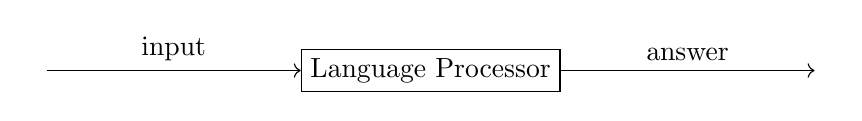
\begin{tikzpicture}
\node (a) at (-5,0) {};
\node (b) at (0,0) [shape=rectangle, draw] {Language Processor};
\node (c) at (5,0) {};

\draw [->] (a) -- (b) node [midway, above] {input} ;
\draw [->] (b) -- (c) node [midway, above] {answer} ;
%\draw [->] (b) -- (c) node [midway, above, text width=3cm, align=center] {improved\\code} ;
\end{tikzpicture}
 \caption[Formal language processor]{A formal language process is fed some input and it returns one of two answers: The input is a valid statement in the language or The input is not a valid statement in the language.}
  \label{F.formal.language.processor}
\end{figure}
%----------------------------------------------------------

If you attempted to create a Language Processor for English, it should probably reject statements like, ``Cup sky red Perl''. But could you create a processor that accepts all valid English (including English poetry), and rejects all non-English. To get a sense of the difficulty of this challenge, I refer you to poetry (considered valid English poetry by those who get to decide such things) by ee cummings (capitalization is correct). 

Those who study formal languages usually restrict themselves to very simple languages. As an example, consider the language of all strings consisting of any combination of the letters ``a'' and ``b''. This language includes strings such as ``aaaa'' and ``abababbbb''. It isn't useful for anything outside the study of formal languages, but it is an example of a formal language.

The study of formal languages is tightly coupled with mathematical sets. In particular, a formal language is a set of strings. Namely, all those strings that meet the definition of the language.  This book assumes you are familiar with mathematical sets including the operations union, intersection, and subtraction. If you aren't familiar with these operations, I'm sure there's a Wikipedia page that can help you out.

Formal languages consist of the following:
\begin{enumerate}
\item An alphabet: a set of characters that the strings in the language are composed of. The alphabet for a language is often represented by the symbol $\Sigma$.
\item A definition of what strings are in the language.
\end{enumerate}

Let's illustrate with an example. 

\begin{quote}
$\Sigma = \{ a b \}$

All strings of five letters.
\end{quote}

Given this definition, the string ``aaxbb'' would be rejected because 'x' is not in the alphabet. The string ``aabb'' would likewise be rejected because it consists of four letters, not five. However, the strings, ``aaaaa'', ``aabbb'', and ``ababa'' would all be included in the language (along with many others).

Formal languages can be broken into categories based on the mechanism used to specify the language. We will initially be interested in three types of definitions, which are discussed in the following chapters.
\begin{enumerate}
\item Recursive definitions (not to be confused with Recursive Languages discussed in Chapter~\ref{C.Beyond.Context.Free})
\item Regular Expressions
\item Context Free Grammars
\end{enumerate}

\chapter{Recursive Definitions}
Recursion is a useful technique in writing some computer programs. It is also a useful technique in specifying formal languages. Consider the following two definitions of the set EVEN:
\begin{enumerate}
\item The set of all positive integers divisible by 2
\item A recursive definition:
\begin{enumerate}
\item 2 is in EVEN
\item If $x$ is in EVEN then $x+2$ is in EVEN.
\end{enumerate}
\end{enumerate}

Which of these two definitions is the most useful? Probably the first one. If you wanted to prove the 96 is in EVEN using the first definition, a simple division by 2 suffices. If you wanted to prove this using the second definition, it would take a bit longer. But there are other instances where a recursive definition is quite elegant.

Consider the following non-recursive definition of arithmetic expressions:
\begin{enumerate}
\item $\Sigma = \{ number\ +\ -\ *\ /\ (\ ) \}$
\item Can't have two operators in a row
\item Must have balanced parenthesis
\item Can't have two numbers in a row
\item Can't begin or end with an operator
\end{enumerate}

Is this set of rules sufficient? Do they allow every valid arithmetic expression? Do the preclude every invalid expression? Could you argue from these rules that the following is a valid arithmetic expression?
\begin{quote}
$(2+7)/3-(((4+5)*(6)-1)*3 + 4)$
\end{quote}
How about:
\begin{quote}
$()()(2+7)/3-(((4+5)*(6)-1)*3 + 4)$
\end{quote}
This last expression meets the definition given above, but is not a valid arithmetic expression because of the empty parenthesis. We could attempt to enhance our list of rules, but how could we know that we have a complete set?

Let's instead give a recursive definition:

\begin{enumerate}
\item Any number is in AE
\item If $f$ and $g$ are in AE, then so are:
\begin{enumerate}
\item $f + g$
\item $f - g$
\item $f * g$
\item $f / g$
\item $(f)$
\end{enumerate}
\end{enumerate}

How can we use this definition to prove an expression is a valid arithmetic expression. We do so by construction: invoke the various rules one at a time until the desired expression is constructed. Let's do so with the expression:
\begin{quote}
$(2+7)/5$
\end{quote}
The construction is as follows:
\begin{enumerate}
\item $2$ is in AE (Rule 1)
\item $7$ is in AE (Rule 1)
\item $2+7$ is in AE (Points 1 and 2 and Rule 2b)
\item $(2+7)$ is in AE (Point 3 and Rule 2e)
\item $5$ is in AE (Rule 1)
\item $(2+7)/5$ is in AE (Points 4 and 5 and Rule 2d)
\end{enumerate}
Having constructed the desired expression using the rules, we have proven that it is a valid arithmetic expression. (More formally, we have proven that it is in the language AE as defined above).

How do we prove that an expression isn't in AE? This is a bit more complicated. Take the expression given above:
\begin{quote}
$()()(2+7)/3-(((4+5)*(6)-1)*3 + 4)$
\end{quote}
Let's generalize it to the statement:
\begin{quote}
Valid statements in AE never have empty parenthesis.
\end{quote}

Before proving this statement, we will prove a different one:
\begin{quote}
Valid statements in AE never start with a close parenthesis and never end with an open parenthesis.
\end{quote}
The proof is as follows:
\begin{enumerate}
\item Numbers do not contain parenthesis, so Rule~1 cannot create an AE that starts with a close parenthesis or ends with an open parenthesis.
\item If $f$ and $g$ do not start with a close parenthesis or end with an open parenthesis, none of the Rule 2's will create a string that starts with a close parenthesis or ends with an open parenthesis.
\item Since there is no way to construct a string that starts with a close parenthesis or ends with an open parenthesis, such a string does not exist in AE.
\end{enumerate}

Back to empty parenthesis: We could prove this using a similar mechanism to what we just used. However, we will use proof by contradiction just to illustrate this mechanism. With this style of proof, you assume the opposite of what you want to prove and then reason until you encounter a contradiction. Since you got to a contradiction, your assumption must have been false. Note: as we will see later, it is important that you only make a single assumption. The contradiction means at least one of your assumptions was false. If you've made multiple assumptions, you don't know which one is false.

Let's assume that a string in AE can contain empty parenthesis. Let's define $s$ as the shortest string that contains empty parenthesis. The string $s$ must be constructed using one of the rules. Which one? Let's consider them one at a time:
\begin{enumerate}
\item Numbers do not contain parenthesis, so $s$ cannot be constructed using Rule~1.
\item The empty string is not a valid number. Rules 2a-2e add characters to the string, and no rules subtract characters from the string. Therefore, it is not possible to have an empty string in AE.
\item Rules 2a-2d do not add parenthesis to the string so they cannot create $s$.
\item Rule 2e will create an empty set of parenthesis if either:
\begin{enumerate}
\item $f$ is the empty string 
\item $f$ begins with a close parenthesis or ends with an open parenthesis
\end{enumerate}
However, we've already proven that neither of these can happen.
\item Since there is no way to construct $s$, are assumption must be false: A string in AE cannot contain empty parenthesis.
\end{enumerate}

\section{Constructing Recursive Definitions}
We've seen several recursive definitions. What do they have in common? A recursive definition is always composed of two parts:
\begin{itemize}
\item Base Cases that identify some set of strings in the language. The base case for AE was ``Any number is in AE''.
\item Recursive Rules of the form, ``If $x$ is in L, the so is $f(x)$''. Rules 2a-2e for AE are the recursive rules. 
\end{itemize}

When constructing recursive definitions, it is important to keep in mind what the language is. For example, the language AE was a set of strings. As a result, rules 2a-2e were adding characters to the string, they were not performing arithmetic operations. The language EVEN was a set of numbers. As a result, Rule~b was performing an arithmetic operation to create a new number.

If the language is a set of strings, then the recursive rules always extend or combine strings. That is, they always make longer strings, they never remove characters from the string. In other words, you should never have a rule of the form, ``If $x$ in in L, then so is $x$ without the trailing semicolon.''

\section{Summary}
Recursive definitions provide a mechanism to construct formal languages. A recursive definition consists of base cases and recursive rules that are used to extend the language. The mechanism we presented here isn't very mathematically rigorous, so we can't prove many properties about the languages that are generated by these definitions (a short-coming that won't be found in the next several chapters). One thing we can say about languages generated by recursive definitions is that they are always infinte. That is, they always contain an infinite number of words. This is true because there is not limit on how many times a recursive rule can be invoked, and each invocation produces a new word in the language.
\needsproblems{}

\part{Regular Languages}
\chapter{Regular Expressions}
Many programmers are familiar with regular expressions from non-compiler contexts. Examples include using an asterisk (*) as a wildcard in a file name, or specifying patterns for the \code{grep} utility. Different programs use different syntax for specifying regular expressions. In this chapter a minimalist syntax for all regular expressions is presented. Most programs that interpret regular expressions enhance this syntax in various ways to make writing regular expressions easier, but the added syntax does not add extra capabilities. In this chapter, we are not interested in programs that make use of regular expressions, so we don't need the syntactic sugar that many of the add. Instead, we are interested in the formal languages that can be specified using regular expressions.

Regular expressions include the following features:
\begin{mydesc}[10em]
	\item[Concatenation] Concatenation is gluing two strings end-to-end. For example, concatenating ``\code{ab}'' with ``\code{bc}'' yields the string ``\code{abcd}''.
  \item[Alternation] Alternation means to choose exactly one from a set of alternatives. Regular expressions use either the vertical bar (\code{|}) or the plus sign (\code{+}) to mean alternation. So the expression \code{a | b | c} means to choose either an '\code{a}', a '\code{b}', or a '\code{c}'. 
	\item[Grouping] Parenthesis can be used for grouping operations much as they can in algebraic expressions.
	\item[Kleene Closure] Kleene Closure means to take zero or more instances of a string. Kleene Closure is denoted by an asterisk (\code{*}). So, for example, \code{x*} means zero or more '\code{x}' characters. Kleene Closure has higher precedence than concatenation so that \code{ab*} means \code{a(b*)} not \code{(ab)*}.
\end{mydesc}

In addition to these operations, the $\Lambda$ symbol is used to represent an empty string (a string with no characters in it).

The most common enhancements to this syntax are as follows:
\begin{mydesc}
\item[zero or one] The question mark
 (\code{?}) 
indicates zero or one of an item so that \code{a?} 
means the same as ($\Lambda$ \code{| a}).
\item[one or more] The plus sign (\code{+}) is similar to Kleene Closure, but it is one-or-more not zero-or-more so that \code{a+} means the same as \code{aa*}.
\item[character range] Square brackets (\code{[]}) can be used to specify a character range so that \code{[a-m]} means any single character in the range '\code{a}' through '\code{m}'. This could be represented long-hand as '\code{(a | b | c | d | ...)}'.
\end{mydesc}

If we want a regular expression for integer constants, we could try
\begin{quote}\code{[0-9]+}\end{quote}
but this allows any number of leading zeros. A better expression would be:
\begin{quote}\code{[1-9][0-9]*}\end{quote}
This fixes the leading zero problem, but it does not allow the number zero. This can be fixed as follows:
\begin{quote}\code{0 | ([1-9][0-9]*)}\end{quote}
If we want to allow negative numbers, we could add an optional minus sign:
\begin{quote}\code{0 | (-?[1-9][0-9]*)}\end{quote}

The following exercises can be used to practice writing regular expressions. You use the enhanced syntax or the minimal syntax for these exercises.

\textbf{Exercises}

\begin{enumerate}
\item Write a regular expression for a string containing any odd number of the letter \code{a}.
\item Write a regular expression for C (or Java) variable names. Valid characters include upper and lower case letters, digits, and the underscore (\code{\_}).
\item Write a regular expression for a string containing any number (including zero) of a positive even number of \code{a}'s followed by an add number of \code{b}'s. The following are valid strings: \code{aaaabbb}, \code{aabaabaabbb}, \code{aaaaaabbbbbaabaabaab}. The following are not valid strings: \code{aaab}, \code{aaaabbbaa}, \code{bbbaab}.
\item For the previous question, state why each of the non-valid strings are non-valid.
\item Write a regular expression for a floating-point constant. The following rules apply: 
\begin{enumerate}
\item The integer part cannot have leading zeros unless the integer part is zero. 
\item If there is a decimal point, it must be followed by at least one digit.
\item The decimal part must not have trailing zeros unless the decimal part is zero.
\end{enumerate}
\end{enumerate}

\section{Language Families}
Each regular expression defines a language.\footnote{These languages are not unique; it is possible to write multiple regular expressions for the same language.} Remember that a formal language is a set of strings. Also recall that it is possible to have a set of sets, so what can we say about the set of all languages that can be defined by regular expressions? This set is known as Regular Languages. They are ``regular'' in the sense that they can be defined by a regular expression. Regular languages have a set of properties that they share. We will eventually explore what these properties are. 

Separate from the set of regular languages, there is the language of regular expressions. We can give a recursive definition of this language (but we cannot give a regular expression for it because, as we shall see, it is not regular).

\begin{enumerate}
\item Every letter in $\Sigma$ is in RE
\item If $r_1$ and $r_2$ are in RE, the so are:
\begin{enumerate}
\item $r_1 r_2$
\item $r_1 + r_2$
\item $r_1*$
\item $(r_1)$
\end{enumerate}
\end{enumerate}

So we now have three separate but related languages:
\begin{itemize}
\item The language (set of all strings) defined by a particular regular expression.
\item The set of all languages definable by regular expressions.
\item The set of all regular expressions.
\end{itemize}

It is important to keep these three languages separate. Consider the following questions, one for each category of language:
\begin{itemize}
\item What is the language defined by \code{(a | b)*a(a | b)*}? This question is asking you to enumerate (or otherwise describe) a particular regular language.
\item Is the language L regular? This is asking whether the specific language L is in the set of all languages definable by regular expressions.
\item Is the statement, '\code{a | (b | c)+} a regular expression? This is asking ``Is it a well-formed regular expression?'' or ``Is it in the language for regular expressions that we gave a recursive definition for?''
\end{itemize}

Any language that can be defined by a regular expression is known as a regular language. In the coming sections we want to examine properties of regular languages (properties of the entire family of regular languages, not of a particular regular language. We will do a couple of them now.

First of all, how do you prove a language is regular? The obvious solution is to write a regular expression that generates the language. One needs to be careful to make sure the regular language actually generates the correct language. For example, if one asked, ``Is the language of all strings over $\Sigma = \{a b\}$ which contain at least one \code{a} and at least one \code{b} regular?''
 the regular expression
\begin{quote}
\code{(a+b)*a(a+b)*b(a+b)*}
\end{quote}
would not be proof that it was. All strings generated by this regular expression contain at least one \code{a} and at least one \code{b}, but the string \code{ba} is part of the language, but it cannot be generated by the regular expression.

A regular expression that generates a language is adequate proof that the language is regular (provided the regular expression actually corresponds to the language). How can we prove a language isn't regular? An inability to write a regular expression for the language is not sufficient proof. The statement, ``I can't write a regular expression for that language'' might be because the language isn't regular or it might be because you simply aren't creative (or smart or persistent) enough to come up with one. We will Have to wait awhile before we can come up with a proof that a language isn't regular.

Theorem~\ref{TH.finite.languages} gives the first property we will prove regarding regular languages.
\begin{theorem}
\label{TH.finite.languages}
All finite languages are regular.
\end{theorem}

The proof is quite simple. If a language is finite, every word in the language can be enumerated. The list might be very long, but it can be generated. A regular expression that corresponds to this language is simply the alternation of each word in the language:
\begin{quote}
(word\_1) + (word\_2) + \dots + (word\_n)
\end{quote}

\section{Why Regular Languages?}
We've identified a class of languages known as ``Regular Languages'' --- namely, those languages that can be defined by regular expressions. Why is this class of languages interesting? From a theory point of view, they are interesting because they form what is considered the smallest class of mathematically defined formal languages. Later chapters will deal with larger classes of languages which are supersets of regular languages. 

From a practical point of view, regular languages are useful because fast an efficient to process. By ``process'', what is meant is answering the question, ``Is this input a member of a particular regular language?'' A common application of this is the \code{grep} utility included with most Linux distributions. With \code{grep}, you specify a regular expression and an input file, and \code{grep} identifies all lines of the file that include a match for the regular expression\footnote{This is a simplification of what \code{grep} does, but it is accurate for the purposes of this illustration}. Most uses of regular expressions include ``scanning'' for a match. A text string (often the contents of a text file) is read looking for a match to the regular expression. How efficient are regular expressions scanners? Theorem~\ref{TH.O.N.for.res}, which won't be proven until later, gives a bound on their efficiency.
\begin{theorem}
\label{TH.O.N.for.res}
Any regular expression can be scanned for in $O(N)$ with small time constant where $N$ is the length of the input string.
\end{theorem}

The next chapter discusses a ``machine'' that can perform this processing.

\chapter{Finite Automata}
There is a well-known children's game called Chutes and Ladders. The goal is to be the first player to move their piece from the beginning (bottom) to the ending (top) of the board. On a player's turn, they spin a spinner which lands on a number. The player advances their piece the specified number of squares on the board. If their piece lands on the bottom of a ladder, they climb the ladder thus making extra progress towards their goal. If their piece lands on the top of a chute, they slide down the chute winding up closer to the beginning. This game is considered a ``children's'' game because it involves no strategy. The outcome of the game is completely determined by the sequence of numbers generate by the spinner (assuming the players don't cheat).

What does this game have to do with regular expressions of finite automata? If we assume that the spinner only generates numbers less than ten (single digit numbers), then we could spin the spinner a bunch of times and write down each result. The result would be a string of digits. We could then ask the question, ``Does this sequence of moves result in someone winning the game?'' That still doesn't sound like a regular expression question (although scanning a string sounds familiar), so let's think of a state machine.

A state machine consists of a finite number of states (or configurations) and transitions from state to state. How could we turn Chutes and Ladders into a state machine? Suppose there were three players. Each player's marker could be on any of the squares on the board. Each configuration of markers (each player on each valid square in every combination) could be considered a state. There would be a large number of states, but the number would be finite. Transitions consist of moves: for example, Player~2 moves forward three spaces. Each state would have an outbound transition for each possible spinner result for each player. We now have a state machine representation of the game, but the question still remains, ``What does this have to do with regular expressions?''

Before we answer that question (through some other examples), lets define a standardized way of graphically representing state machines (or more formally, finite automata). Finite Automata (aka State Machines) consist of a finite number of states and transitions between states. One state is defined as the start state, and any number of states can be defined as final states. The start state in an FA is signified by an inbound arrow that doesn't originate from another state. Processing always starts in the start state. Final states are signified by a double circle. Transitions are labeled by the letter that is used to move from one state to another. This format is illustrated in Figure~\ref{F.FA_1}.

%----------------------------------------------------------
\begin{figure}[hbt]
\centering
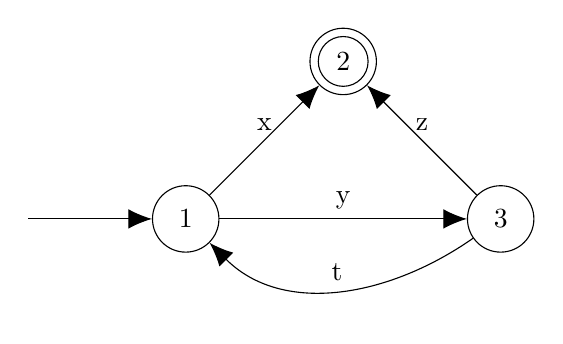
\begin{tikzpicture}

\fastart {-4, -2};
\fanonterminalnode {-2,-2}{1};
\faterminalnode {0,0}{2};
\fanonterminalnode {2,-2}{3};

\fatransition{start}{1}{};
\fatransition{1}{2}{x};
\fatransition{1}{3}{y};
\fatransition{3}{2}{z};
\faarctransition {3}{1}{t}{215}{315};

\end{tikzpicture}
 \caption[Sample Finite Automaton]{This is a sample FA. State~1 is the start state (it has an incoming arrow from nowhere). State~2 is a final state (signified by the double-circle). The transitions are labeled by what letter is used to move from one state to another.}
  \label{F.FA_1}
\end{figure}
%----------------------------------------------------------

Using the FA in Figure~\ref{F.FA_1}, and the input $ytx$, the processing starts in State~1 (the start state). The $y$ is used to transition to State~3. The $t$ is used to transition back to State~1. The $x$ is used to transition to State~2. Since the input is exhausted while in a final state, the string is accepted by the FA.

Two conditions can cause a string to be rejected: 
\begin{enumerate}
\item If the input is exhausted and the current state isn't a final state. The input $yty$ illustrates this case.
\item If there is no outbound transition on the current letter. The input $yx$ illustrates this case.
\end{enumerate}

Given these rules for processing FA's, it should be clear that the FA in Figure~\ref{F.FA_1} is equivalent to the regular expression \code{(yt)* (x | yz)}. It is no coincidence that there is a regular expression that corresponds to the FA. It turns out that every FA is equivalent to some regular expression, and that each regular expression has an FA that is equivalent to it. We will prove this in a later section.

Figure~\ref{F.FA_2} gives another FA. This FA shows a slightly different format. The start state has a '-' in the label. Final states have a '$+$' in them. The states can be though of as follows:
\begin{enumerate}
\item State 1: the start state.
\item State 2: An $a$ not preceded by an $a$.
\item State 3: A $b$ not preceded by a $b$.
\item State 4: Have read a double letter.
\end{enumerate}
Note that once a double letter has been found, the FA remains in the final state no matter what other letters are read.

%----------------------------------------------------------
\begin{figure}[hbt]
\centering
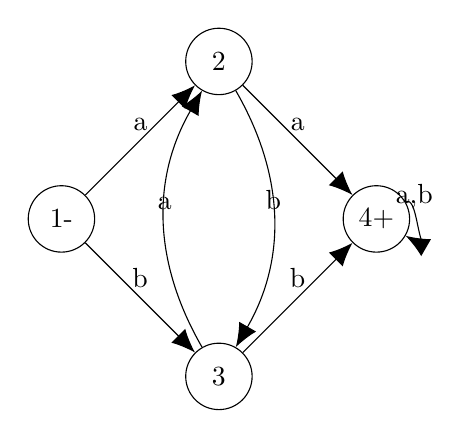
\begin{tikzpicture}

\fanonterminalnode {-2,0}{1-};
\fanonterminalnode {2,0}{4+};
\fanonterminalnode {0,2}{2};
\fanonterminalnode {0,-2}{3};

\fatransition{1-}{2}{a};
\fatransition{1-}{3}{b};
\fatransition{2}{4+}{a};
\fatransition{3}{4+}{b};
\faarctransition{3}{2}{a}{120}{240};
\faarctransition {2}{3}{b}{300}{60};
\faarctransition {4+}{4+}{a,b}{30}{330};

\end{tikzpicture}
 \caption[FA for double letters]{This FA accepts all strings that contain a double letter.}
  \label{F.FA_2}
\end{figure}
%----------------------------------------------------------

FA's can also be represented in table form. These tables are called transition tables. The transition table for the FA in Figure~\ref{F.FA_2} is given in Figure~\ref{T.FA.2}. There is one row for each state. The state name is given in the first column. The remaining columns indicate the new state based on the transition letter at the top of the column.

%----------------------------------------------------------
\begin{figure}[hbt]
\centering
\begin{tabular}{|c|c|c|}
\hline
Current State & a & b \\
\hline
1- & 2 & 3 \\
\hline
2 & 4 & 3 \\
\hline
3 & 2 & 4 \\
\hline
4+ & 4 & 4 \\
\hline
\end{tabular}
\caption[Transition Table]{This transition table represents the same FA as Figure~\ref{F.FA_2}}
\label{T.FA.2}
\end{figure}

\section{Non-deterministic Finite Automata}

The FA illustrated in Figure~\ref{F.FA_1} is a Deterministic Finite Automaton (DFA). It is deterministic in the sense that for each character that is processed, the FA has exactly one choice on what to do. There is another class of FA's known as Non-deterministic Finite Automata (NFA's). With NFA's, for a given input, there is the potential for multiple choices on what to do. The choices can take two forms:
\begin{enumerate}
\item Multiple outbound edges labeled with the same letter. If that letter is read, any of the outbound edges labeled with that letter can be taken. This is illustrated by the edges from Node~$a$ labeled $z$ in Figure~\ref{F.NFA_1}.
\item Edges labeled $\Lambda$. These edges can be taken without consuming an input character. Node~$a$ has a $\Lambda$ transition meaning you can leave Node~$a$ without consuming any characters.
\end{enumerate}

%----------------------------------------------------------
\begin{figure}[hbt]
\centering
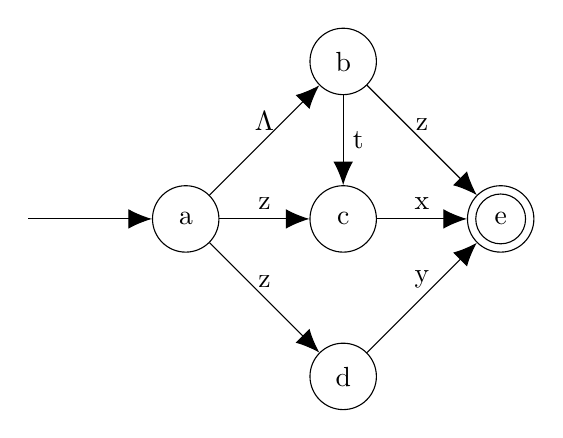
\begin{tikzpicture}

\fastart {-4, 0};
\fanonterminalnode {-2,0}{a};
\fanonterminalnode {0,2} {b};
\fanonterminalnode {0,0} {c};
\fanonterminalnode {0,-2} {d};
\faterminalnode {2,0} {e};

\fatransition{start}{a}{};
\fatransition{a}{b}{$\Lambda$};
\fatransition{a}{c}{z};
\fatransition{a}{d}{z};
\fatransition{b}{e}{z};
\farighttransition{b}{c}{t};
\fatransition{c}{e}{x};
\fatransition{d}{e}{y};

\end{tikzpicture}
 \caption[Sample Non-deterministic Finite Automaton]{This is a sample NFA. Node $a$ has multiple outbound transitions on $z$. It also has an outbound transition on $\Lambda$ meaning you could leave Node~$a$ without consuming any characters.}
  \label{F.NFA_1}
\end{figure}
%----------------------------------------------------------

The NFA in Figure~\ref{F.NFA_1} accepts the following stings:
\begin{mydesc}[2em]
	\item[$z$] This string is accepted by following the $\Lambda$ transition to Node~$b$ and then using the $z$ to transition to Node~$e$.
	\item[$tx$] This string is accepted by following the $\Lambda$ transition to Node~$b$ and then using the $t$ to transition to Node~$c$ and the $x$ to transition to Node~$e$.
	\item[$zx$] This string is accepted by using the $z$ to transition to Node~$c$ and then using the $x$ to transition to Node~$e$.
	\item[$zy$] This string is accepted by using the $z$ to transition to Node~$d$ and then using the $y$ to transition to Node~$e$.
\end{mydesc}

NFA's aren't any more powerful than DFA's--anything you can do with an NFA you can also do with a DFA\footnote{Section~Figure~\ref{S.Subset.Construction} gives a construction that can turn any NFA into an equivalent DFA. This is sufficient to argue that anything that can be done with an NFA can also be done with a DFA.}. The reason for introducing NFA's is that converting from a regular expression to code that accepts strings matching that regular expression makes use of NFA's.

\section{Thompson's}

The first step in converting a regular expression to executable code is to convert it to an equivalent NFA. For this conversion, we are going to use Thompson's Construction\footnote{Credited to Ken Thompson, the originator of the Unix operating system.}. The beauty of Thompson's construction is that it is a mechanical process -- one that doesn't require any creative thought. In other words, it can be automated. A computer program can be written to perform this conversion.

%----------------------------------------------------------
\begin{figure}[htb]
\centering

%\scalebox{.7}{
\begin{subfigure}[b]{0.45\textwidth}
\centering
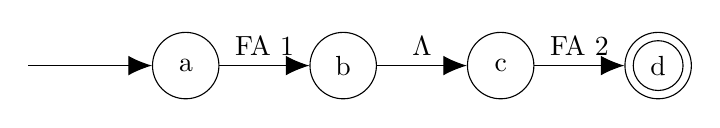
\begin{tikzpicture}
\fastart {0, 0};
\fanonterminalnode {2,0} {a};
\fanonterminalnode {4,0} {b};
\fanonterminalnode {6,0} {c};
\faterminalnode {8,0} {d};

\fatransition{start}{a}{};
\fatransition{a}{b}{FA 1};
\fatransition{b}{c}{$\Lambda$};
\fatransition{c}{d}{FA 2};

%\node at (5,-1) {Concatenation};
%\node at (5,-2) {};
\end{tikzpicture}
\caption{Concatenation}\label{F.Thompsons.Concatenation}
\end{subfigure}
%}

%\scalebox{.7}{
\begin{subfigure}[b]{0.45\textwidth}
\centering
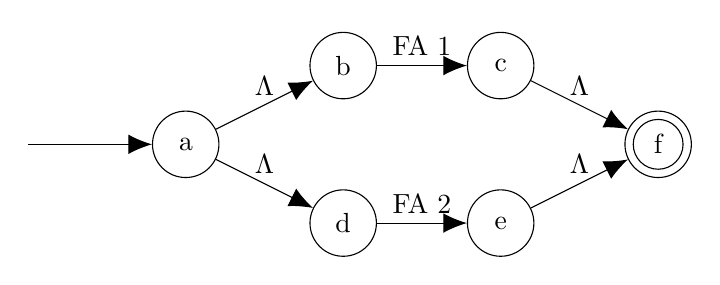
\begin{tikzpicture}
\fastart {0, 0};
\fanonterminalnode {2,0} {a};
\fanonterminalnode {4,1} {b};
\fanonterminalnode {6,1} {c};
\fanonterminalnode {4,-1} {d};
\fanonterminalnode {6,-1} {e};
\faterminalnode {8,0} {f};

\fatransition{start}{a}{};
\fatransition{a}{b}{$\Lambda$};
\fatransition{b}{c}{FA 1};
\fatransition{c}{f}{$\Lambda$};

\fatransition{a}{d}{$\Lambda$};
\fatransition{d}{e}{FA 2};
\fatransition{e}{f}{$\Lambda$};
%\node at (5,-2) {Alternation};
%\node at (5,-3) {};
\end{tikzpicture}
%}
\caption{Alternation}\label{F.Thompsons.Alternation}
\end{subfigure}

%\scalebox{.7}{
\begin{subfigure}[b]{0.45\textwidth}
\centering
%Kleene Closure
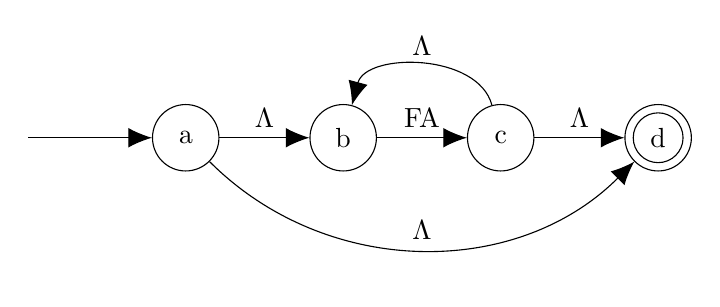
\begin{tikzpicture}
\fastart {0, 0};
\fanonterminalnode {2,0} {a};
\fanonterminalnode {4,0} {b};
\fanonterminalnode {6,0} {c};
\faterminalnode {8,0} {d};

\fatransition{start}{a}{};
\fatransition{a}{b}{$\Lambda$};
\fatransition{b}{c}{FA};
\fatransition{c}{d}{$\Lambda$};
\faarctransition {a}{d}{$\Lambda$}{315}{225};
\faarctransition {c}{b}{$\Lambda$}{105}{75};

%\node at (5,-2) {Kleene Closure};
%\node at (5,-3) {};
\end{tikzpicture}
%}
\caption{Kleene Closure}\label{F.Thompsons.KleeneClosure}
\end{subfigure}

 \caption[Thompson's Construction]{Thompson's Construction method makes use of these three diagrams. For each diagram, the FA(s) being composed are represented as two nodes (the start and end nodes) labeled $FA$, $FA 1$, or $FA 2$.}
  \label{F.Thompsons}
\end{figure}
%----------------------------------------------------------

If two FA's each have a single start state and a single final state, and if the start state doesn't have any inbound edges and the final state doesn't have any outbound edges, then the two FA's can be composed by connecting the end state of one FA to the start state of the other using a $\Lambda$ transition. Thompson's Construction makes use of this fact by creating composed FA's for each operation supported by regular expressions (concatenation, alternation, and Kleene Closure). An NFA can be built for any regular expression simply by composing it one small piece at a time using Thompson's three diagrams. Figure~\ref{F.Thompsons} shows the three base diagrams.

The trick to using Thompson's construction is to NOT be creative. Each FA built with Thompson's has a single start and a single final state. The diagram can be dropped as-is directly into the next step in the construction. Nodes never need to be erased, and each composition should be drawn exactly as shown in Figure~\ref{F.Thompsons}.

Let's illustrate by doing several constructions. First, let's construct an NFA for \code{a (b | c)}. It's best to start with the inner most operation (in this case \code{(b | c)}) and work out. So first draw the alternation diagram as shown below:

\begin{center}
\scalebox{.7}{
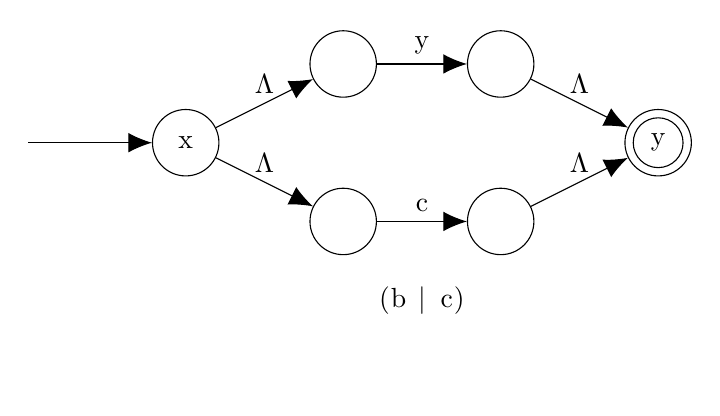
\begin{tikzpicture}
\fastart {0, 0};
\fanonterminalnode {2,0} {x};
\fanolabel {4,1} {b1};
\fanolabel {6,1} {b2};
\fanolabel {4,-1} {c1};
\fanolabel {6,-1} {c2};
\faterminalnode {8,0} {y};

\fatransition{start}{x}{};
\fatransition{x}{b1}{$\Lambda$};
\fatransition{b1}{b2}{y};
\fatransition{b2}{y}{$\Lambda$};

\fatransition{x}{c1}{$\Lambda$};
\fatransition{c1}{c2}{c};
\fatransition{c2}{y}{$\Lambda$};

\node at (5,-2) {\code{(b | c)}};
\node at (5,-3) {};
\end{tikzpicture}
} % end scaled box
\end{center}
The resulting diagram gets dropped into the \code{FA 2} position of the concatenation diagram as illustrated below. Note how the node labeled $x$ in the above diagram is in the location of the node labeled $c$ in the concatenation diagram, and the $y$ node is in the $d$ position.

\begin{center}
\scalebox{.7}{
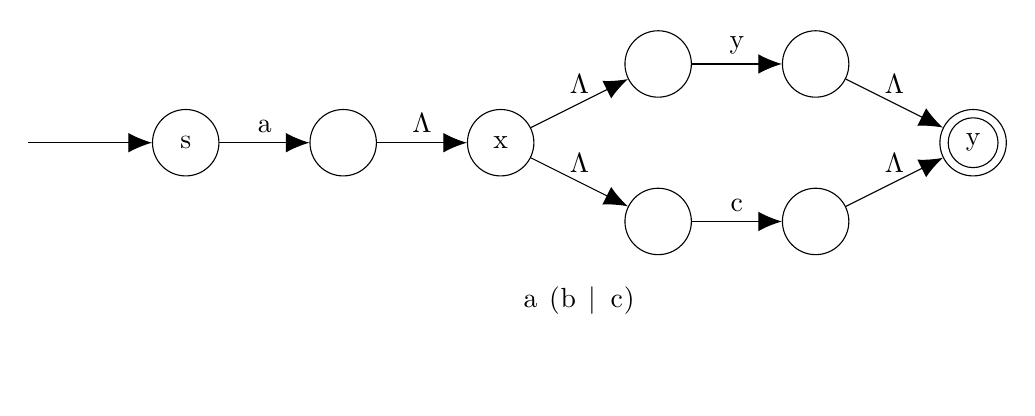
\begin{tikzpicture}
\fastart {0, 0};
\fanonterminalnode {2,0} {s};
\fanolabel {4,0} {a1};

\fanonterminalnode {6,0} {x};
\fanolabel {8,1} {b1};
\fanolabel {10,1} {b2};
\fanolabel {8,-1} {c1};
\fanolabel {10,-1} {c2};
\faterminalnode {12,0} {y};

\fatransition{start}{s}{};
\fatransition{s}{a1}{a};
\fatransition{a1}{x}{$\Lambda$};


\fatransition{x}{b1}{$\Lambda$};
\fatransition{b1}{b2}{y};
\fatransition{b2}{y}{$\Lambda$};

\fatransition{x}{c1}{$\Lambda$};
\fatransition{c1}{c2}{c};
\fatransition{c2}{y}{$\Lambda$};

\node at (7,-2) {\code{a (b | c)}};
\node at (7,-3) {};
\end{tikzpicture}
} % end scalebox
\end{center}

As a second example, let's construct an NFA for \code{a (b | c)*}. This is the same as the previous example, except that the alternation is wrapped in Kleene Closure. The alternation is, again, the innermost operation, and it is the same as in the previous example:

\begin{center}
\scalebox{.7}{
\begin{tikzpicture}
\fastart {0, 0};
\fanonterminalnode {2,0} {x};
\fanolabel {4,1} {b1};
\fanolabel {6,1} {b2};
\fanolabel {4,-1} {c1};
\fanolabel {6,-1} {c2};
\faterminalnode {8,0} {y};

\fatransition{start}{x}{};
\fatransition{x}{b1}{$\Lambda$};
\fatransition{b1}{b2}{y};
\fatransition{b2}{y}{$\Lambda$};

\fatransition{a}{c1}{$\Lambda$};
\fatransition{c1}{c2}{c};
\fatransition{c2}{y}{$\Lambda$};

\node at (5,-2) {\code{(b | c)}};
%\node at (5,-3) {};
\end{tikzpicture}
} % end scaled box
\end{center}

This is now dropped into the Kleene Closure construction:

\begin{center}
\scalebox{.7}{
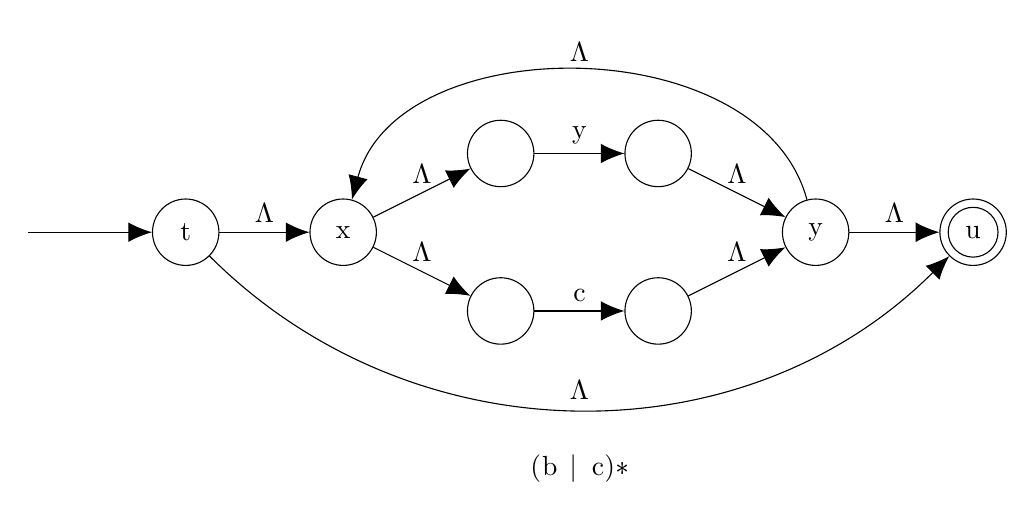
\begin{tikzpicture}
\fastart {0, 0};
\fanonterminalnode {2,0} {t}
\fanonterminalnode {4,0} {x};
\fanolabel {6,1} {b1};
\fanolabel {8,1} {b2};
\fanolabel {6,-1} {c1};
\fanolabel {8,-1} {c2};
\fanonterminalnode {10,0} {y};
\faterminalnode {12,0} {u};

\fatransition{start}{t}{};
\fatransition{t}{x}{$\Lambda$};
\fatransition{x}{b1}{$\Lambda$};
\fatransition{b1}{b2}{y};
\fatransition{b2}{y}{$\Lambda$};

\fatransition{x}{c1}{$\Lambda$};
\fatransition{c1}{c2}{c};
\fatransition{c2}{y}{$\Lambda$};

\fatransition{y}{u}{$\Lambda$};

\faarctransition {t}{u}{$\Lambda$}{315}{225};
\faarctransition {y}{x}{$\Lambda$}{105}{75};

\node at (7,-3) {\code{(b | c)*}};
\end{tikzpicture}
} % end scaled box
\end{center}

Finally, we drop this into the concatenation construction:
\begin{center}
\scalebox{.7}{
\begin{tikzpicture}
\fastart {0, 0};
\fanonterminalnode {2,0} {a}
\fanonterminalnode {4,0} {t}
\fanonterminalnode {6,0} {x};
\fanolabel {8,1} {b1};
\fanolabel {10,1} {b2};
\fanolabel {8,-1} {c1};
\fanolabel {10,-1} {c2};
\fanonterminalnode {12,0} {y};
\faterminalnode {14,0} {u};

\fatransition{start}{s}{};
\fatransition{s}{t}{$\Lambda$};
\fatransition{t}{x}{$\Lambda$};
\fatransition{x}{b1}{$\Lambda$};
\fatransition{b1}{b2}{y};
\fatransition{b2}{y}{$\Lambda$};

\fatransition{x}{c1}{$\Lambda$};
\fatransition{c1}{c2}{c};
\fatransition{c2}{y}{$\Lambda$};

\fatransition{y}{u}{$\Lambda$};

\faarctransition {t}{u}{$\Lambda$}{315}{225};
\faarctransition {y}{x}{$\Lambda$}{105}{75};

\node at (8,-3) {\code{a (b | c)*}};
\end{tikzpicture}
} % end scaled box
\end{center}

As a third example, \code{a* (b | c)}, includes a concatenation of two complex item (\code{a*} and \code{(b | c)} ). To construct this, first construct \code{a*}, then construct \code{(b | c)} and then use the concatenation construction to combine them. Here are the results:

\begin{center}
\scalebox{.7}{
\begin{tikzpicture}
\fastart {0, 0};
\fanonterminalnode {2,0} {t};
\fanolabel {4,0} {b};
\fanolabel {6,0} {c};
\fanonterminalnode {8,0} {u};

\fatransition{start}{t}{};
\fatransition{t}{b}{$\Lambda$};
\fatransition{b}{c}{a};
\fatransition{c}{u}{$\Lambda$};
\faarctransition {a}{u}{$\Lambda$}{315}{225};
\faarctransition {c}{b}{$\Lambda$}{105}{75};

\fanonterminalnode {10,0} {x};
\fanolabel {12,1} {b1};
\fanolabel {14,1} {b2};
\fanolabel {12,-1} {c1};
\fanolabel {14,-1} {c2};
\faterminalnode {16,0} {y};

\fatransition{u}{x}{$\Lambda$};
\fatransition{x}{b1}{$\Lambda$};
\fatransition{b1}{b2}{y};
\fatransition{b2}{y}{$\Lambda$};

\fatransition{x}{c1}{$\Lambda$};
\fatransition{c1}{c2}{c};
\fatransition{c2}{y}{$\Lambda$};

\node at (8,-2) {\code{a* (b | c)}};
%\node at (5,-3) {};
\end{tikzpicture}
} % end scaled box
\end{center}

It should be clear that Thompson's construction creates lots of $\Lambda$ transitions. This begs the question, ``isn't there an simpler way to draw these?''. The answer is in two parts. If by ``simpler'' you mean ``easier construction'', my answer would be ``no''. The whole point of Thompson's construction is that it is a simple mechanical process. It requires no creative thought. But if by ``simpler'' you mean a less complex result (one without all the $\Lambda$s), then the answer is ``yes''. The next section gives an algorithm to convert these complex NFAs into DFAs (diagrams without any $\Lambda$ transitions. The goal is not to make the diagram simpler, the goal is to get a DFA because they are easier to process in code.

\section{Subset Construction}\label{S.Subset.Construction}

To illustrate how an NFA could be processed, let's consider again the NFA for \code{a* (b | c)} presented in the last section, but presented again in Figure~\ref{F.subsetNFA}. In this figure, each node is labeled so they can be explicitly referred to. For each state, we can ask the question, ``What states could I wind up in if I encounter a particular letter in the input?''. For example, suppose we haven't consumed any input yet, what states could we be in? Clearly we could be in State~$1$, the start state, but because of the $\Lambda$ transitions, we could also be in states $2, 4, 5, 6, 8$. This set of states ($=\{1, 2, 4, 5, 6, 8\}$)\footnote{When specifying sets of characters,  it is often easier to read the list of items if each item is separated with a comma. This works unless the set included a comma (as sets of characters for a compiler often do). I will generally included commas for readability unless the set of characters includes punctuation (commas or other punctuation marks). I hope this will improve readability.}
forms a meta-state (let's call it $A$). From the meta-state~$A$, where could we wind up if we read an $a$. Since the meta-state~$A$ includes state~$2$, we can follow the $a$ to state~$3$. From there we can follow $\Lambda$s to $2, 4, 5, 6, 8$. This gives another meta-state. Let's call it $B = \{2, 3, 4, 5, 6, 8\}$. 

\begin{figure}[hbt]
\centering
\scalebox{.7}{
\begin{tikzpicture}
\fastart {0, 0};
\fanonterminalnode {2,0} {1};
\fanonterminalnode {4,0} {2};
\fanonterminalnode {6,0} {3};
\fanonterminalnode {8,0} {4};

\fatransition{start}{1}{};
\fatransition{1}{2}{$\Lambda$};
\fatransition{2}{3}{a};
\fatransition{3}{4}{$\Lambda$};
\faarctransition {a}{4}{$\Lambda$}{315}{225};
\faarctransition {3}{2}{$\Lambda$}{105}{75};

\fanonterminalnode {10,0} {5};
\fanonterminalnode {12,1} {6};
\fanonterminalnode {14,1} {7};
\fanonterminalnode {12,-1} {8};
\fanonterminalnode {14,-1} {9};
\faterminalnode {16,0} {10};

\fatransition{4}{5}{$\Lambda$};
\fatransition{5}{6}{$\Lambda$};
\fatransition{6}{7}{b};
\fatransition{7}{10}{$\Lambda$};

\fatransition{5}{8}{$\Lambda$};
\fatransition{8}{9}{c};
\fatransition{9}{10}{$\Lambda$};

\end{tikzpicture}
} % end scaled box
\caption[NFA produced by Thompson's]{This is the NFA produced by Thompson's for the regular expression \code{a* (b | c)}}
  \label{F.subsetNFA}
\end{figure}

We could continue to find new meta-states by enumerating all possible outbound inputs from each meta-state and then following the $\Lambda$s from the resulting states. The results are presented in Table~\ref{T.subsetTable1}.

\begin{table}[hbt]
\center
\begin{tabular}{l|l|l|l}
\hline
\textbf{meta-state} & \textbf{NFA states} & \textbf{input} & \textbf{resulting states} \\
\hline
A & 1, 2, 4, 5, 6, 8 & a & 2, 4, 5, 6, 8 \\
A & 1, 2, 4, 5, 6, 8 & b & 7, 10 \\
A & 1, 2, 4, 5, 6, 8 & c & 9, 10 \\
B & 2, 4, 5, 6, 8 & a & 2, 4, 5, 6, 8 \\
B & 2, 4, 5, 6, 8 & b & 7, 10 \\
B & 2, 4, 5, 6, 8 & c & 9, 10 \\
C & 7, 10 & a & - \\
C & 7, 10 & b & - \\
C & 7, 10 & c & - \\
D & 9, 10 & a & - \\
D & 9, 10 & b & - \\
D & 9, 10 & c & - \\
\hline
\end{tabular}
\caption[Result of subset construction]{The results of performing the subset construction on the NFA in Figure~\ref{F.subsetNFA}. An input of ``-'' means there are no valid inputs starting from this state. Resulting states of ``-'' mean there are no valid destinations from this state.}
\label{T.subsetTable1}
\end{table}

We need a formal algorithm for producing these tables. The steps are as follows:
\begin{enumerate}
\item From the start state, follow all $\Lambda$s. Follow as many as you can, not just one. This is known as the $\Lambda$ closure of a state: all states reachable from a given state following only $\Lambda$s. This set of states is labeled $A$ in the table.
\item Make multiple rows, one for each character in the source-language, for each meta-state not already in the table. Initially this is only meta-state~$A$, and for the example NFA in Figure~\ref{F.subsetNFA}, the characters in the source language are $a, b, c$ meaning three rows for each meta-state.
\item For each NFA state in the meta-state, if there is an outbound transition on the input, write down the destination state in the resulting states column.
\item Extend the list of states in the resulting states column by forming the $\Lambda$ closure of each state already in the column.
\item If there are any new unique sets of states in the resulting states column, give them a unique label and return to Step~2.
\end{enumerate}
The process will stop once all existing rows are filled in and no new rows get generated.

Let's use these rules to derive a table for the NFA below. Note: this NFA was \textbf{not} generated with Thompson's.

\begin{center}
\scalebox{.7}{
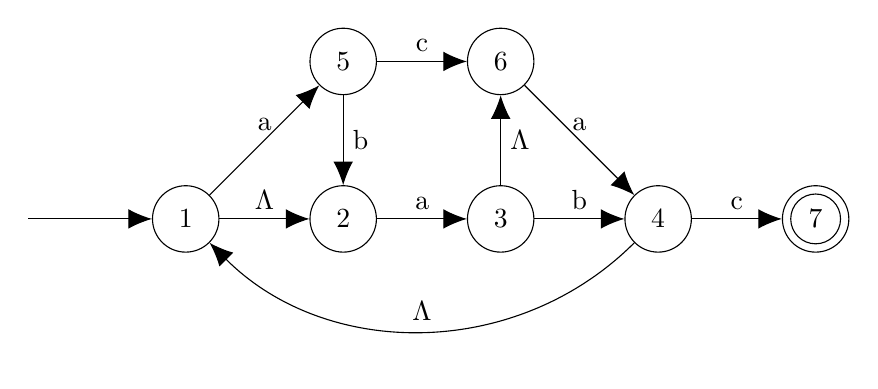
\begin{tikzpicture}
\fastart {0, 0};
\fanonterminalnode {2,0} {1};
\fanonterminalnode {4,0} {2};
\fanonterminalnode {6,0} {3};
\fanonterminalnode {8,0} {4};
\fanonterminalnode {4,2} {5};
\fanonterminalnode {6,2} {6};
\faterminalnode {10,0} {7};

\fatransition{start}{1}{};
\fatransition{1}{2}{$\Lambda$};
\fatransition{2}{3}{a};
\fatransition{3}{4}{b};
\farighttransition{3}{6}{$\Lambda$};
\fatransition{4}{7}{c};
\fatransition{1}{5}{a};
\fatransition{5}{6}{c};
\farighttransition{5}{2}{b};
\fatransition{6}{4}{a};
\faarctransition {4}{1}{$\Lambda$}{225}{315};

\end{tikzpicture}
} % end scaled box
\end{center}

Step~1 yields states 1 and 2, so this set becomes meta-state-$A$. There are three letters in the source language (a, b, c), so this yields the following rows:

\begin{center}
\small
\begin{tabular}{l|l|l|l}
\hline
\textbf{meta-state} & \textbf{NFA states} & \textbf{input} & \textbf{resulting states} \\
\hline
A & 1, 2 & a &  \\
A & 1, 2 & b &  \\
A & 1, 2 & c &  \\
\hline
\end{tabular}
\end{center}

Completing the first row, we can follow an $a$ from state 1 to 5, and from state 2 to 3. Add these two states to the resulting states column, and then follow the $\Lambda$s adding state 6. Label the set \code{ \{3, 5, 6\}} as meta-state~$B$ and add rows to the table:

\begin{center}
\small
\begin{tabular}{c|l|l|l|l}
\hline
& \textbf{meta-state} & \textbf{NFA states} & \textbf{input} & \textbf{resulting states} \\
\hline
1 & A & 1, 2 & a & B = 3, 5, 6 \\
2 & A & 1, 2 & b &  \\
3 & A & 1, 2 & c &  \\
4 & B & 3, 5, 6 & a &  \\
5 & B & 3, 5, 6 & b &  \\
6 & B & 3, 5, 6 & c &  \\

\hline
\end{tabular}
\end{center}

Completing rows 2 and 3, there are no $b$ nor $c$ transitions out of any of the states in meta-state~$A$, so the resulting states for both of these rows are empty.

Moving on to row 4, we can follow an $a$ from state 6 to state 4. We can then follow $\Lambda$s from 4 to 1 and 1 to 2 yielding meta-state $C$ containing states 1, 2, 4.

\begin{center}
\small
\begin{tabular}{c|l|l|l|l}
\hline
& \textbf{meta-state} & \textbf{NFA states} & \textbf{input} & \textbf{resulting states} \\
\hline
1 & A & 1, 2 & a & B = 3, 5, 6 \\
2 & A & 1, 2 & b & - \\
3 & A & 1, 2 & c & - \\
4 & B & 3, 5, 6 & a & C = 1, 2, 4 \\
5 & B & 3, 5, 6 & b & \\
6 & B & 3, 5, 6 & c & \\
7 & C & 1, 2, 4 & a & \\
8 & C & 1, 2, 4 & b & \\
9 & C & 1, 2, 4 & c & \\
\hline
\end{tabular}
\end{center}

For row 5, we can follow a $b$ from 3 to 4 and from 5 to 2. There are no $\Lambda$s from either 2 or 4, so meta-state~$D$ contains 2 and 4.

For row 6, we can follow a $c$ from 5 to 6. There are no $\Lambda$s from 6, so meta-state~$E$ contains only 6. Adding these new rows to the table, we have:

\begin{center}
\small
\begin{tabular}{c|l|l|l|l}
\hline
& \textbf{meta-state} & \textbf{NFA states} & \textbf{input} & \textbf{resulting states} \\
\hline
1 & A & 1, 2 & a & B = 3, 5, 6 \\
2 & A & 1, 2 & b & - \\
3 & A & 1, 2 & c & - \\
4 & B & 3, 5, 6 & a & C = 1, 2, 4 \\
5 & B & 3, 5, 6 & b & D = 2, 4 \\
6 & B & 3, 5, 6 & c & E = 6 \\
7 & C & 1, 2, 4 & a & \\
8 & C & 1, 2, 4 & b & \\
9 & C & 1, 2, 4 & c & \\
10 & D & 2, 4 & a & \\
11 & D & 2, 4 & b & \\
12 & D & 2, 4 & c & \\
13 & E & 6 & a & \\
14 & E & 6 & b & \\
15 & E & 6 & c & \\
\hline
\end{tabular}
\end{center}

Completing row 10, we can follow an $a$ from 1 to 5 and 2 to 3. The $\Lambda$ closure adds 6. This set of states is already labeled $B$, so we don't need to add any rows to the table.

For Row 11, there are no outbound edges on $b$ so the resulting states is empty.

For Row 12, we can follow a $c$ from 4 to 7. This new meta-state is labeled $F$.

\begin{center}
\small
\begin{tabular}{c|l|l|l|l}
\hline
& \textbf{meta-state} & \textbf{NFA states} & \textbf{input} & \textbf{resulting states} \\
\hline
1 & A & 1, 2 & a & B = 3, 5, 6 \\
2 & A & 1, 2 & b & - \\
3 & A & 1, 2 & c & - \\
4 & B & 3, 5, 6 & a & C = 1, 2, 4 \\
5 & B & 3, 5, 6 & b & D = 2, 4 \\
6 & B & 3, 5, 6 & c & E = 6 \\
7 & C & 1, 2, 4 & a & B\\
8 & C & 1, 2, 4 & b & -\\
9 & C & 1, 2, 4 & c & F = 7 \\
10 & D & 2, 4 & a & \\
11 & D & 2, 4 & b & \\
12 & D & 2, 4 & c & \\
13 & E & 6 & a & \\
14 & E & 6 & b & \\
15 & E & 6 & c & \\
16 & F & 7 & a & \\
17 & F & 7 & b & \\
18 & F & 7 & c & \\
\hline
\end{tabular}
\end{center}

For row 10, we can follow the a from 2 to 3 and then the $\Lambda$ to 6. This is meta-state~$G$.

For row 11, there are no outbound transitions on $b$, so the resulting states is empty.

For row 12, we can follow a $c$ from 4 to 7. This is already labeled $F$.

\begin{center}
\small
\begin{tabular}{c|l|l|l|l}
\hline
& \textbf{meta-state} & \textbf{NFA states} & \textbf{input} & \textbf{resulting states} \\
\hline
1 & A & 1, 2 & a & B = 3, 5, 6 \\
2 & A & 1, 2 & b & - \\
3 & A & 1, 2 & c & - \\
4 & B & 3, 5, 6 & a & C = 1, 2, 4 \\
5 & B & 3, 5, 6 & b & D = 2, 4 \\
6 & B & 3, 5, 6 & c & E = 6 \\
7 & C & 1, 2, 4 & a & B\\
8 & C & 1, 2, 4 & b & -\\
9 & C & 1, 2, 4 & c & F = 7 \\
10 & D & 2, 4 & a & G = 3, 6\\
11 & D & 2, 4 & b & - \\
12 & D & 2, 4 & c & F \\
13 & E & 6 & a & \\
14 & E & 6 & b & \\
15 & E & 6 & c & \\
16 & F & 7 & a & \\
17 & F & 7 & b & \\
18 & F & 7 & c & \\
19 & G & 3, 6 & a & \\
20 & G & 3, 6 & b & \\
21 & G & 3, 6 & c & \\
\hline
\end{tabular}
\end{center}

For Row 13, we can follow an $a$ from 6 to 4 and then $\Lambda$s to 1 and 2. This is already labeled $C$.

For Rows 13-18, there are no available outbound transitions, so the resulting states are empty.

The transitions for Row 19 are the same as for Row 13, so the result is $C$.

For Row 20, we can follow a $b$ from 3 to 4 and then $\Lambda$s give us meta-state $C$.

For Row 21, there are no outbound transitions on $c$ so the resulting state is empty.

This gives us the following table:

\begin{center}
\small
\begin{tabular}{c|l|l|l|l}
\hline
& \textbf{meta-state} & \textbf{NFA states} & \textbf{input} & \textbf{resulting states} \\
\hline
1 & A & 1, 2 & a & B = 3, 5, 6 \\
2 & A & 1, 2 & b & - \\
3 & A & 1, 2 & c & - \\
4 & B & 3, 5, 6 & a & C = 1, 2, 4 \\
5 & B & 3, 5, 6 & b & D = 2, 4 \\
6 & B & 3, 5, 6 & c & E = 6 \\
7 & C & 1, 2, 4 & a & B\\
8 & C & 1, 2, 4 & b & -\\
9 & C & 1, 2, 4 & c & F = 7 \\
10 & D & 2, 4 & a & G = 3, 6\\
11 & D & 2, 4 & b & - \\
12 & D & 2, 4 & c & F \\
13 & E & 6 & a & C\\
14 & E & 6 & b & - \\
15 & E & 6 & c & - \\
16 & F & 7 & a & - \\
17 & F & 7 & b & - \\
18 & F & 7 & c & - \\
19 & G & 3, 6 & a & C \\
20 & G & 3, 6 & b & C\\
21 & G & 3, 6 & c & - \\
\hline
\end{tabular}
\end{center}

All rows are filled in, so we are done.

\textbf{Important note:} The procedure is to follow the input out of the NFA states and then follow the $\Lambda$s. A common mistake is to follow the $\Lambda$s out of the NFA states. For example, when filling out the last row, even though there is a $\Lambda$ from state 3, we don't follow it because we are only looking for transitions on $c$.

The subset construction was supposed to turn an NFA into a DFA, but it appears to have just produced a table. We can take the information in our final table from the example we just completed and summarize it in Figure~\ref{F.transitionTable}.

%----------------------------------------------------------
\begin{figure}[hbt]
\centering

\small
\begin{tabular}{l|l|l}
\hline
\textbf{From} & \textbf{transition on} & \textbf{To} \\
\hline
A & a & B \\
B & a & C \\
B & b & D \\
B & c & E \\
C & a & B\\
C & c & F \\
D & a & G \\
D & c & F \\
E & a & C\\
G & a & C \\
G & b & C\\
\hline
\end{tabular}
\caption[Transition table for DFA]{A summary of the table derived in this section. Each row contains the start state, and input character, and the resulting state if that character is found while in the start state.}
  \label{F.transitionTable}
\end{figure}
%----------------------------------------------------------

This is known as a transition table. It is fairly straight forward to convert this table into a DFA (and a DFA into a transition table). Create states for each state in the table (the union of the From and To columns). The start state is always $A$, and any meta-state that included a final state in the original NFA is a final state in the DFA (in this case State~$F$). The resulting DFA is as follows:

\begin{center}
\scalebox{.7}{
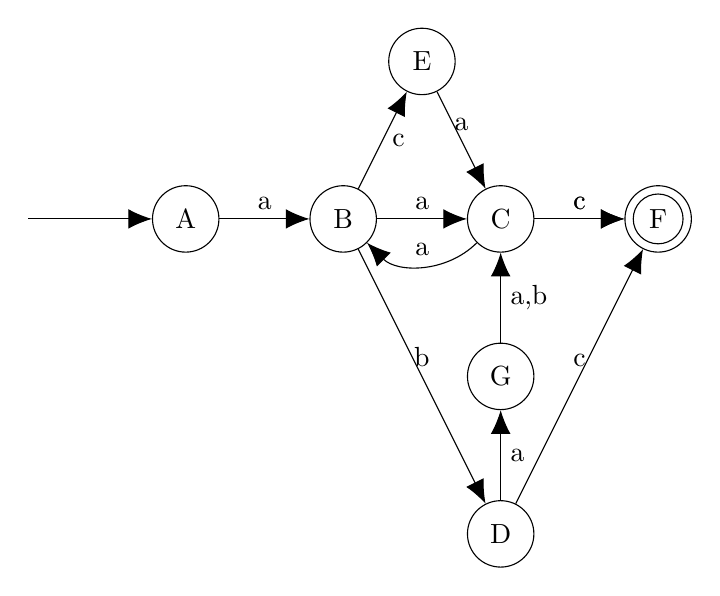
\begin{tikzpicture}
\fastart {0, 0};
\fanonterminalnode {2,0} {A};
\fanonterminalnode {4,0} {B};
\fanonterminalnode {6,0} {C};
\fanonterminalnode {6,-4} {D};
\fanonterminalnode {5,2} {E};
\faterminalnode    {8,0} {F};
\fanonterminalnode {6,-2} {G};

\fatransition{start}{A}{};
\fatransition{A}{B}{a};
\fatransition{B}{C}{a};
\fatransition{C}{F}{c};
\fatransition{C}{F}{c};
%\faarctransition{B}{D}{b}{270}{180};
\fatransition{B}{D}{b};
\farighttransition{D}{G}{a};
\farighttransition{G}{C}{a,b};
%\faarctransition{D}{F}{c}{0}{270};
\fatransition{D}{F}{c};
\farighttransition{B}{E}{c};
\fatransition{E}{C}{a};
\faarctransition {C}{B}{a}{225}{315};

\end{tikzpicture}
} % end scaled box
\end{center}

Does the subset construction always result in a DFA, or might it result in another NFA? The answer is that it always results in a DFA for the following two reasons:
\begin{enumerate}
\item The \emph{input} column never has $\Lambda$s, so the resulting FA will not have any $\Lambda$ transitions.
\item When generating rows, each meta-state has exactly one row for each input character. As a result, there will never be multiple outbound transitions for the same character.
\end{enumerate}
The consequence is that the resulting FA has no non-determinism and is therefore a DFA.

\chapter{Theory}

What we have done so far:

We have shown that Thompson's Construction can turn any regular expression into an NFA. This implies that:
\begin{quote}
$L($regular expressions$) \subseteq L($NFA$)$
\end{quote}
This statement means that the set of all languages that can be constructed with regular expressions is a subset (or equal) of the languages that can be constructed with an NFA. In other words, anything that can be done with a regular expression can also be done with an NFA.

The Subset Construction showed that any NFA can be turned into a DFA. This implies that:
\begin{quote}
$L($NFA$) \subseteq L($DFA$)$
\end{quote}
So we now have:
\begin{quote}
$L($regular expressions$) \subseteq L($NFA$) \subseteq L($DFA$)$
\end{quote}

There are proofs both by induction and construction that show that any DFA can be turned into a regular expression. The proofs aren't particularly illuminating, so they won't be presented here. The statement will simply be taken on faith. So we now have:

\begin{quote}
$L($regular expressions$) \subseteq L($NFA$) \subseteq L($DFA$) \subseteq L($regular epxressions$)$
\end{quote}
The only way that this can be true is if:
\begin{quote}
$L($regular expressions$) = L($NFA$) = L($DFA$)$
\end{quote}
In other words, regular expressions, NFAs and DFAs are all equally powerful. They can be used to define exactly the same set of languages. This relation is known as Kleene's Theorem. It can be used to prove interesting properties of regular languages. 

\begin{theorem}
The union of two regular languages is regular.
\end{theorem}
This can be proved by construction. Consider two languages $L_1$ and $L_2$ both of which are regular. Since they are regular, there is a DFA that corresponds to each of them. If we construct a new NFA by creating a new start state that is connected to the start states of both $L_1$ and $L_2$, we would have an NFA that accepts any word in $L_1$ or any word in $L_2$. Since we have an NFA for this language, the language must be regular.
\needswork


\begin{theorem}
The intersection of two regular languages is regular.
\end{theorem}

zzz
\part{Context Free Grammars}
\chapter{Context Free Grammars}
\needswork{}

\chapter{Context Free Grammars}
Regular expressions are used to define the tokens a compiler processes. We also need a mechanism to define the syntax of the language a compiler processes. Context Free Grammars are used for this purpose.

A Context Free Grammar (CFG) is made up a a list of productions of the form:

\indent this symbol can be replaced by this collection of symbols

A production in a CFG consists of a left hand side and a right hand side. The left hand side gives the symbol that can be replaced. The right hand side gives the list of symbols that can replace the symbol on the left. The two sides are typically separated 
either by an arrow ( $\rightarrow$ ) 
or sometimes a colon-colon-equals ( ::= ). 
A sample production that indicates that the symbol \code{A} 
can be replaced by \code{X Y Z} is given below:

\cfgprod{A}{X Y Z}

Symbols in CFGs are of two flavors: non-terminals are those that appear on the left hand side of a production. They are non-terminals because they can be replaced by other symbols. Terminals are those symbols that never appear on the left hand side. They are ``terminal'' because they can never be replaced. For ease of reading, non-terminals are usually given in UPPERCASE. terminals are given in lowercase. CFGs also need a start symbol - the symbol that is the starting point for derivations. The start symbol is often either \code{S} or \code{START}, but if neither is specified, the left hand side of the first production is considered the start symbol.

%----------------------------------------------------------
\begin{cfg}{A CFG that defines the language of any number of \code{a}'s followed by the same number of \code{b}'s.}{F.cfg.1}
Q\cfgprod{S}{a S b}Q
Q\cfgprod{S}{$\lambda$}Q
\end{cfg}
%----------------------------------------------------------

Figure~\ref{F.cfg.1} shows a complete CFG. The productions have been numbered for easy reference. There are only two productions. The first one says that the start symbol (\code{S}) can be replaced with \code{a S b}. Note that this is a recursive rule because the \code{S} appears on both sides. The second production says that \code{S} can be replaced with nothing.

What can we do with this CFG? Let's do some derivations. Starting with the start symbol and Production 1, we can get the string \code{aSb}. If we then use Production 2, we are left with the string \code{ab}. Since there are no more non-terminals, we are done.

What if we invoked Production 1 more than once? The first invocation produces \code{aSb}. The next invocation produces \code{aaSbb}. Each invocation adds another \code{a} and \code{b}. When we finally invoke Production 2, we are left with a string of \code{a}'s followed by the same number of \code{b}'s.

While not the most complex illustration, this CFG illustrates that CFGs are more powerful than regular expressions. Regular expressions are not able to generate balanced parenthesis. A regular expression such as \code{(*)*} allows any number of opening parenthesis and any number of closing parenthesis, but there is no way to guarantee that the number of closing parenthesis match the number of opening parenthesis. If we substituted parenthesis for the \code{a} and \code{b} in Figure~\ref{F.cfg.1}, we would have a solution to the balanced parenthesis problem.

Figure~\ref{F.cfg.2} presents a more complete, and more interesting CFG. This language defines a program as zero or more statements. An individual statement can be an assignment statement (in this language, an assignment statement is a terminal, so the assumption is that they are defined elsewhere), an \code{if} statement, or a compound statement (curly braces surrounding any number of statements). 

%----------------------------------------------------------
\begin{figure}[hbt]
\centering
\begin{enumerate}
\item \cfgprod{PROGRAM}{STMTS}
\item \cfgprod{STMTS}{STMT STMTS}
\item \cfgprod{STMTS}{$\lambda$}
\item \cfgprod{STMT}{IF\_STMT}
\item \cfgprod{STMT}{COMPOUND\_STMT}
\item \cfgprod{STMT}{assignment\_stmt}
\item \cfgprod{IF\_STMT} {if ( expr ) STMT}
\item \cfgprod{COMPOUND\_STMT} { \{ STMTS \} }
\item \cfgprod{COMPOUND\_STMT} { STMT }
\end{enumerate}
\caption[CFG of a simple programming language]{This CFG defines a program as being zero or more statements, where each statement is either an \code{if} statement, an assignment statement or a compound statement.}
\label{F.cfg.2}
\end{figure}
%----------------------------------------------------------

\begin{lstlisting}[caption={Sample program in the language defined by the CFG in Figure~\ref{F.cfg.2}},label=L.nested.ifs]
assignment_statement
if (expr)
   assignment_statement
if (expr)
    if (expr)
       assignment_statement
if (expr)
{
   assignment_statement
   assignment_statement
   {
   }
}
\end{lstlisting}

The program in Listing~\ref{L.nested.ifs} illustrates the features of the language defined by the CFG in Figure~\ref{F.cfg.2}. Line~1 is a simple assignment statement. The \code{if} statement that begins in Line~2 is a simple \code{if} statement. The \code{if} statement that begins in Line~4 shows a nested \code{if} statement. The compound statement that begins in Line~8 shows that compound statements can be nested and that they can be empty (in Line~11).

\section{Derivations}

Listing~\ref{L.nested.ifs} claims to be a program in the language defined in Figure~\ref{F.cfg.2}. How can we substantiate this claim? This is normally done by showing a derivation of the program given the CFG. Each line of a derivation substitutes a single non-terminal for the right-hand-side of a production for that non-terminal. 

Derivations start with the start symbol and continue until there are only non-terminals. Each step other than the first should list the production number that was invoked to make the substitution. Rather than starting with the longer program in Listing~\ref{L.nested.ifs}, let's start with the shorter program in Listing~\ref{L.short.prog}.

\begin{lstlisting}[caption={Short program program in the language defined by the CFG in Figure~\ref{F.cfg.2}. The derivation of this program is given in Derivation~\ref{D.derive.1}},label=L.short.prog]
if (expr)
{
   assignment_statement
   assignment_statement
}
\end{lstlisting}

\begin{derivation}{Derivation of the program in Listing~\ref{L.short.prog}}{D.derive.1}
    PROGRAM
1   STMTS
4   IF_STMT
7   if ( expr ) STMT
8   if ( expr ) { STMTS }
2   if ( expr ) { STMT STMTS }
6   if ( expr ) { assignment_stmt STMTS }
2   if ( expr ) { assignment_stmt STMT STMTS }
6   if ( expr ) { assignment_stmt assignment_stmt STMTS }
3   if ( expr ) { assignment_stmt assignment_stmt }
\end{derivation}

\chapter{Pushdown Automata}
\needswork{}

\part{Beyond Context Free Languages}
\label{C.Beyond.Context.Free}
\needswork{}

\appendix

\chapter{The First Appendix}

The \verb"\appendix" command should be used only once. Subsequent appendices can
be created using the Chapter command.

\chapter{The Second Appendix}

Some text for the second Appendix.

This text is a sample for a short bibliography. You can cite a book by making use of
the command \verb"\cite{KarelRektorys}": \cite{KarelRektorys}. Papers can be cited
similarly: \cite{Bertoti97}. If you want multiple citations to appear in a single set
of square brackets you must type all of the citation keys inside a single citation,
separating each with a comma. Here is an example: \cite{Bertoti97, Szeidl2001,
Carlson67}.

\begin{thebibliography}{9}
\bibitem {KarelRektorys}Rektorys, K., \textit{Variational methods in Mathematics,
Science and Engineering}, D. Reidel Publishing Company,
Dordrecht-Hollanf/Boston-U.S.A., 2th edition, 1975

\bibitem {Bertoti97} \textsc{Bert\'{o}ti, E.}:\ \textit{On mixed variational formulation
of linear elasticity using nonsymmetric stresses and displacements}, International
Journal for Numerical Methods in Engineering., \textbf{42}, (1997), 561-578.

\bibitem {Szeidl2001} \textsc{Szeidl, G.}:\ \textit{Boundary integral equations for
plane problems in terms of stress functions of order one}, Journal of Computational and
Applied Mechanics, \textbf{2}(2), (2001), 237-261.

\bibitem {Carlson67}  \textsc{Carlson D. E.}:\ \textit{On G\"{u}nther's stress functions
for couple stresses}, Quart. Appl. Math., \textbf{25}, (1967), 139-146.
\end{thebibliography}

\backmatter

\chapter{Afterword}

The back matter often includes one or more of an index, an afterword,
acknowledgments, a bibliography, a colophon, or any other similar item. In
the back matter, chapters do not produce a chapter number, but they are
entered in the table of contents. If you are not using anything in the back
matter, you can delete the back matter TeX field and everything that follows it.
\end{document}
